\chapter{Depth Map Prediction using Machine Learning}

Thinking about the original inspiration of our project, human can eaisy estimate the distance between the scenery and themselves, we believe that is based on binocular vision. However, after thinking over, we may find we are not so sure about this hypothesis, because when we close one eye, we can still see the world and we can still estimate the depth of the scenery, maybe a little harder. 

On the other hand, we did plenty of calculations in our projects, including build calibration model, image compare, to get the depth information. But do we really do this kind of calculations in out brain all the time? If the answer is yes, when do we begin to learn this approach? Do we estimate depth information simple based on the two images of left and right view? We may find the answer is no, because so many other cues are used when we estimate the distance of one object. For example, we know that one building should far larger than a person and when a building and a person project to our retina with the same size, we should know the build is far and the person is near to us. 

Actually, our brain do so many amazing things, the brain can learn to process images, sounds, it can learn to process our sense of touch. It seems like if we want to mimic the brain, we have to write lots of different pieces of software and programs. But instead, the way the brain does it is just worth a single learning algorithms, this is a hypothesis and widely accepted by scientists now. This magical algorithm is neural network algorithm. 

Machine learning is a field of computer science that often uses statistical techniques to give computers the ability to "learn" In this chapter, we want to make a machine learn to predict the depth information using neural network, which is a machine learning task.

\section{Convolutional Neural Network}

Convolutional neural networks (CNNs) are the current state-of-the-art model architecture for image classification tasks. CNNs apply a series of filters to the raw pixel data of an image to extract and learn higher-level features, which the model can then use for classification and other iamge processing tasks.

In this section. We build a model to classify the images of hand write number, as shown in Figure \ref{fig:number}. Through studying amount of features, the classifier can label a new iamges with the number on it, the accuracy can reach 0.99.

\begin{figure}[h!]
	\centering
	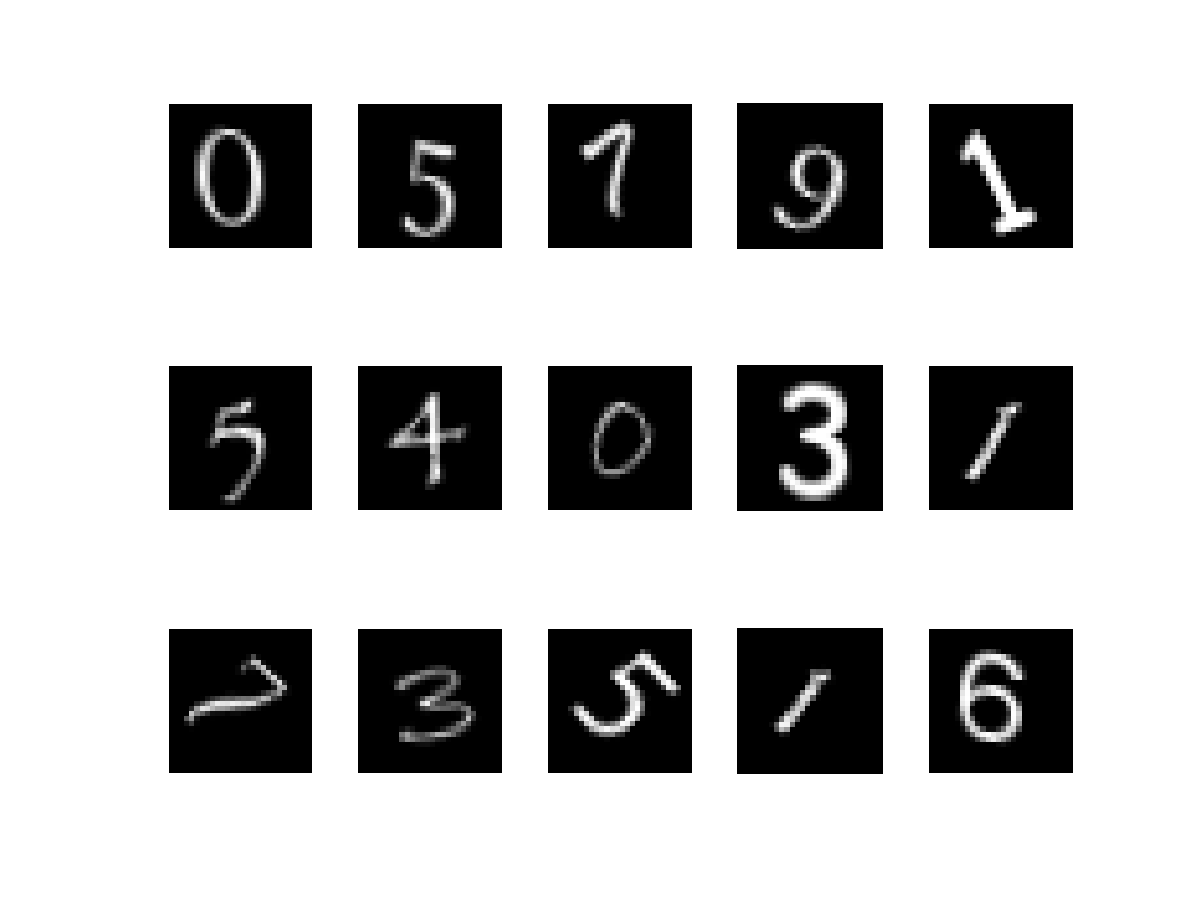
\includegraphics[width=0.8\linewidth]{figures/part3/number}
	\caption{Hand write numbers}
	\label{fig:number}
\end{figure} 

Usually, CNNs contains three components:
\begin{itemize}
	\item Convolutional layers, which apply a specified number of convolution filters to the image. For each subregion, the layer performs a set of mathematical operations to produce a single value in the output feature map.
	\item Pooling layers, which downsample the image data extracted by the convolutional layers to reduce the dimensionality of the feature map in order to decrease processing time. A commonly used pooling algorithm is max pooling, which extracts subregions of the feature map (e.g., 2x2-pixel tiles), keeps their maximum value, and discards all other values. In our model, we use 
	\item Dense (fully connected) layers, which perform classification on the features extracted by the convolutional layers and downsampled by the pooling layers. In a dense layer, every node in the layer is connected to every node in the preceding layer.
\end{itemize}

In our model, we define a deep neural network which contains one input layer, three convolution layers, two pooling layers and a output layer. The result shows deep networks performs better than shallow networks. Figure \ref{fig:train} shows the training progress of our model. From the figure we can easily find the accuracy of classify become higher and higher as the training epoch increase.

\begin{figure}[h!]
	\centering
	\includegraphics[width=0.9\linewidth]{figures/part3/train}
	\caption{Training process}
	\label{fig:train}
\end{figure} 


\section{Stereo ConvNet}

In this section, we introduce a stereo convolution neural network. The network is fully convolutional, and takes a couple of grayscale stereoscopic images concatenated along the channel axis, and ouputs a single image representing the depth map. A series of convolutional and maxpooling layers followed by a series of upscalling and deconvolutional layers allow the network to extract image disparity features at the smaller scale (object edges), and generate a smooth estimate of the depth map at the larger scale (full object). 

Figure \ref{fig:stereo_connet} show the depth map prediction of Stereo ConvNet. The traing/validation sets are created using the random virtual 3d scene generator \footnote{https://github.com/LouisFoucard/DepthMap\_dataset}.

\begin{figure}[h!]
	\centering
	\includegraphics[width=0.8\linewidth]{figures/part3/stereo_connet.pdf}
	\caption{Stereo ConvNet results}
	\label{fig:stereo_connet}
\end{figure} 

 The network is published in \ref .The source code is writen in python use $theano$ library, while I used to use $pyTorch$ and $Tensorflow$ libraries, So I have not implement it by myself in matlab and python. 
